\documentclass[14 pt]{beamer}

\usepackage{hyperref}
\usepackage[utf8]{inputenc}
\usepackage[T1]{fontenc}
\usepackage{microtype}          % ENHANCING READABILITY
\usepackage{lipsum}             % DUMMY TEXT
\usepackage{ccicons}            % ICON SET
\usepackage{mathtools}

% Format presentation size to A4
\setlength{\paperwidth}{29.7cm}
\setlength{\paperheight}{21.0cm}
\setlength{\textwidth}{27.7cm}
\setlength{\textheight}{20.0cm} 

% Fonts
\usepackage[no-math]{fontspec}
\defaultfontfeatures{Mapping=tex-text}
\usepackage{fontawesome5}

% use main font for base text
\usefonttheme{serif}

% font for base text
\setmainfont{Crimson Text}

% font for title
\setbeamerfont{title}{family=\fontspec{Futura Condensed Medium}}
\setbeamerfont{frametitle}{family=\fontspec{Futura Condensed Medium}}
\setbeamerfont{framesubtitle}{family=\fontspec{Crimson Text}}

% for other elements on title page (author, date)
\setbeamerfont{title page}{family=\fontspec{Crimson Text}}

% Color
\definecolor{tempcolor}{RGB}{132,50,5}

\title[Short-title]{TITLE SLIDE\\ \vskip1cm \fontspec{Crimson Text}
\textit{Introduction\\to\\Subtitle}}
\date[ilter-desc]{@hkilter\\ \vskip4cm \ccbyncnd \\ Creative Commons License}
%\date{\today}

\author[ilter]{\textbf{H.~Kem\^al İlter, PhD}}

\usetheme{texsx}

%%%%%%%%%%%%%%%%%%%%%%% TIKZ %%%%%%%%%%%%%%%%%%%%%%%%%%%%%%

%\usepackage{tikz}
\usepackage{pgfplots}
\pgfplotsset{compat=newest}
\usepgfplotslibrary{fillbetween}

\usetikzlibrary{%
  arrows,%
  positioning,
  patterns,
  decorations.pathmorphing,
  calc,
  angles,
  intersections,
  quotes,
  decorations.markings,
  backgrounds
%  shapes.misc,% wg. rounded rectangle
%  shapes.arrows,%
%  chains,%
%  matrix,%
%  positioning,% wg. " of "
%  scopes,%
%  decorations.pathmorphing,% /pgf/decoration/random steps | erste Graphik
%  shadows%
}

%%%%%%%%%%%%%%%%%%%%%%%%%%%%%%%%%%%%%%%%%%%%%%%%%%%%%%%%%%%

\begin{document}

%%%%%%%%%%%%%%%%%%%%%%% COPY & PASTE %%%%%%%%%%%%%%%%%%%%%%

%\begin{frame}[t]
%\frametitle{INDEPENDENCE}
%\framesubtitle{Freedom}
%
%\begin{columns}[t]
%\begin{column}{0.45\textwidth}
%\end{column}
%
%\begin{column}{0.45\textwidth}
%\end{column}
%\end{columns}
%\end{frame}

%%%%%%%%%%%%%%%%%%%%%%%%%%%%%%%%%%%%%%%%%%%%%%%%%%%%%%%%%%%

\begin{frame}
\titlepage
\end{frame}

%%%%%%%%%%%%%%%%%%%%%%%%%%%%%%%%%%%%%%%%%%%%%%%%%%%%%%%%%%%

\begin{frame}[t]
\frametitle{CONTENT}
\framesubtitle{Subtitle}

\begin{columns}[t]
\begin{column}{0.96\textwidth}
\lipsum[1]
\vskip0.5cm%
\lipsum[2]
\end{column}
\end{columns}
\end{frame}

%%%%%%%%%%%%%%%%%%%%%%%%%%%%%%%%%%%%%%%%%%%%%%%%%%%%%%%%%%%

\begin{frame}[t]
\frametitle{CONTENT - TWO COLUMNS}
\framesubtitle{Subtitle}
\begin{columns}[t]
\begin{column}{0.45\textwidth}
\lipsum[3]
\vskip0.5cm%
\lipsum[4]
\end{column}
\begin{column}{0.45\textwidth}
\lipsum[5]
\vskip0.5cm%
\lipsum[6]
\end{column}
\end{columns}
\end{frame}

%%%%%%%%%%%%%%%%%%%%%%%%%%%%%%%%%%%%%%%%%%%%%%%%%%%%%%%%%%%

\begin{frame}[t]
\frametitle{CONTENT WITH FIGURE - TWO COLUMNS}
\framesubtitle{Subtitle}

\begin{columns}[t]
\begin{column}{0.45\textwidth}
\lipsum[7]
\vskip0.5cm%
\lipsum[8]
\end{column}
\begin{column}{0.45\textwidth}
\begin{figure}[t]
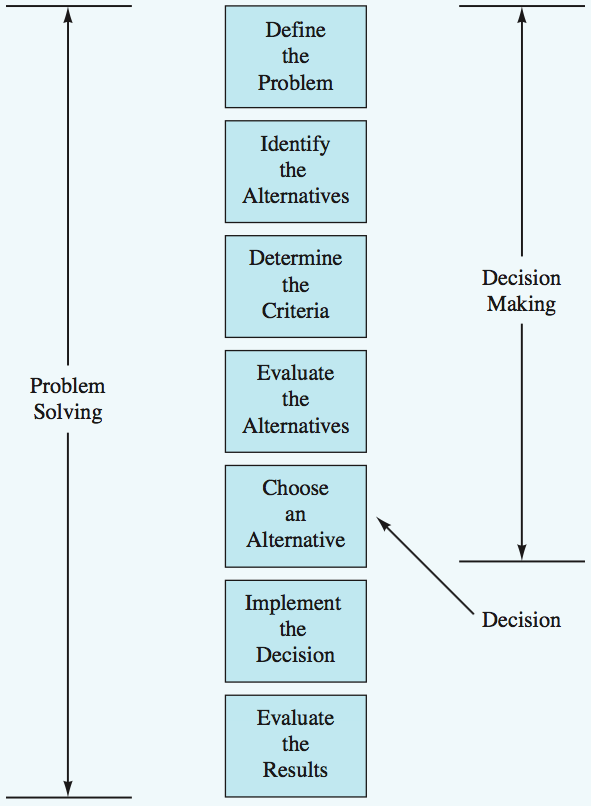
\includegraphics[width=0.7\textwidth]{img/problem-solving-decision-making}
\caption{The relationship between processes of problem solving and decision making.}
\end{figure}

\end{column}
\end{columns}
\end{frame}

%%%%%%%%%%%%%%%%%%%%%%%%%%%%%%%%%%%%%%%%%%%%%%%%%%%%%%%%%%%

\begin{frame}[t]
\frametitle{CONTENT WITH FIGURE - TWO COLUMNS TEXT WITH A WIDE FIGURE}
\framesubtitle{Subtitle}

\begin{columns}[t]
\begin{column}{0.45\textwidth}
\lipsum[8][1-4]
\end{column}

\begin{column}{0.45\textwidth}
\lipsum[9][1-4]
\end{column}
\end{columns}
\vskip1.5cm%
\begin{figure}[t]
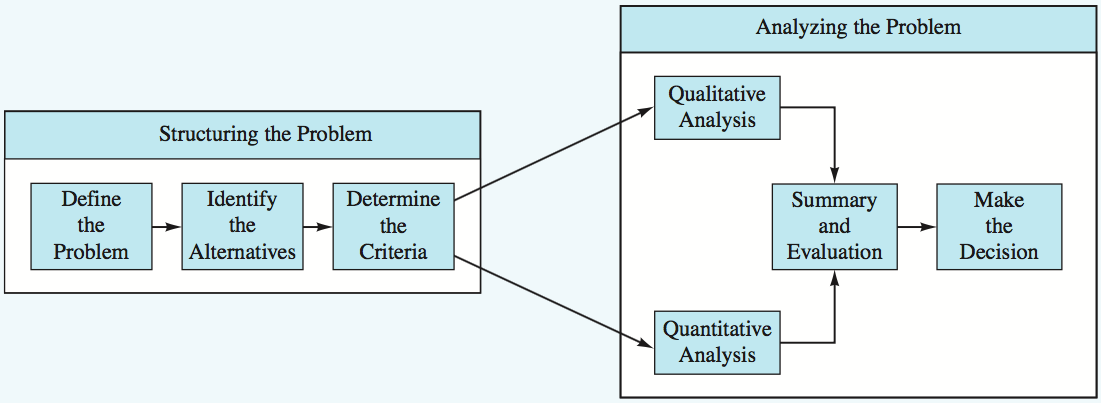
\includegraphics[width=0.7\textwidth]{img/alternate-classification}
\caption{An alternate classification of the decision making process.}
\end{figure}

\end{frame}

%%%%%%%%%%%%%%%%%%%%%%%%%%%%%%%%%%%%%%%%%%%%%%%%%%%%%%%%%%%

\begin{frame}[t]
\frametitle{EXAMPLES}
\framesubtitle{From a Real Presentation}

\begin{columns}[t]
\begin{column}{0.45\textwidth}
Why a quantitative approach might be used in the decision-making process:

\begin{enumerate}
  \item The problem is complex, and the manager cannot develop a good solution without the aid of quantitative analysis.
  \item The problem is especially important (e.g., a great deal of money is involved), and the manager desires a thorough analysis before attempting to make a decision.
  \item The problem is new, and the manager has no previous experience from which to draw.
  \item The problem is repetitive, and the manager saves time and effort by relying on quantitative procedures to make routine decision recommendations.
\end{enumerate}

\end{column}

\begin{column}{0.45\textwidth}
\end{column}
\end{columns}
\end{frame}

%%%%%%%%%%%%%%%%%%%%%%%%%%%%%%%%%%%%%%%%%%%%%%%%%%%%%%%%%%%

\begin{frame}[t]
\frametitle{MODELS}
\framesubtitle{Model Development}

\begin{columns}[t]
\begin{column}{0.45\textwidth}
Models are representations of real objects or situations and can be presented in various forms.
\vskip0.5cm%
\emph{Classification}

\begin{enumerate}
  \item Iconic models, a toy is a physical replica of a real object. 
  \item Analog models, thermometer represents temperature.
  \item Mathematical models, representations of a problem by a system of symbols and mathematical relationships or expressions.
\end{enumerate}
\vskip0.5cm%
\emph{Mathematical Modeling}

A process that translates observed or desired phenomena into mathematical expressions.
\end{column}

\begin{column}{0.45\textwidth}

\end{column}
\end{columns}
\end{frame}

%%%%%%%%%%%%%%%%%%%%%%%%%%%%%%%%%%%%%%%%%%%%%%%%%%%%%%%%%%%

\begin{frame}[t]
\frametitle{MODEL DEVELOPMENT}
\framesubtitle{An Example: Office Furniture Shop}

\begin{columns}[t]
\begin{column}{0.45\textwidth}
\emph{Story}
\vskip0.5cm%
Office Furnature Shop produces three products: Desk, Chair, Molded steel. In the production facility steel as the raw material is used for producing these products. Managers don't worry about the sale process, all products will be sold. We already know two functions from previous slides;
\begin{itemize}
  \item what the total profit of this shop can be at the end of the day, and
  \item how much raw material should be used (required) for production in that day.
\end{itemize}
Company has a warehouse with the capacity of two thousand kilogram and contains steel in it. On that day, managers decide to satisfy expo's contract commitments which are at least hundred desks and at most five hundred chairs.
\begin{table}
\begin{tabular}{p{0.33\textwidth}p{0.33\textwidth}p{0.33\textwidth}}
  \hline
  \emph{Product} & \emph{Profit} & \emph{Raw Steel Used} \\
  \hline
  Desk  & \$50 per item & 7 kg \\
  Chair & \$20 per item & 3 kg\\
  Molded steel & \$6 per kg & 1.5 kg\\
  \hline
\end{tabular}
\caption{Shop's profit for each of products produced.}  
\end{table}
\end{column}

\begin{column}{0.45\textwidth}
\emph{Questions}
\vskip0.5cm%
\begin{itemize}
  \item What are the amounts of products produced to maximize company's profit in that day?
  \item What is the maximum profit of the company at the end of the day?
\end{itemize}
\end{column}
\end{columns}
\end{frame}

%%%%%%%%%%%%%%%%%%%%%%%%%%%%%%%%%%%%%%%%%%%%%%%%%%%%%%%%%%%

\begin{frame}[t]
\frametitle{MODEL DEVELOPMENT}
\framesubtitle{An Example: Office Furniture Shop}

\begin{columns}[t]
\begin{column}{0.45\textwidth}
\emph{Description}
\vskip0.5cm%
There are 3 products to produce: \emph{Desk, Chair, Molded steel}.

No need to think about the sale process, all products will be sold.
\vskip0.5cm%
\emph{Model variables}
\vskip0.5cm%
$D$: Amount of desks (countable, number)\\
$C$: Amount of chairs (countable, number)\\
$M$: Amount of molded steel (uncountable, kg)
\end{column}
\begin{column}{0.45\textwidth}
\emph{Question}
\vskip0.5cm%
What is the \textbf{Total Profit} of this shop at the end of the day?
\end{column}
\end{columns}
\vskip1.5cm%
\begin{table}
\begin{tabular}{p{4cm}p{4cm}}
  \hline
  \emph{Product} & \emph{Profit} \\
  \hline
  Desk  & \$50 per item \\
  Chair & \$20 per item \\
  Molded steel & \$6 per kg \\
  \hline
\end{tabular}

\caption{Shop's profit for each of products produced.}  
\end{table}

\end{frame}

%%%%%%%%%%%%%%%%%%%%%%%%%%%%%%%%%%%%%%%%%%%%%%%%%%%%%%%%%%%

\begin{frame}[t]
\frametitle{MODEL DEVELOPMENT}
\framesubtitle{An Example: Office Furniture Shop}

\begin{columns}[t]
\begin{column}{0.45\textwidth}
\emph{Question}
\vskip0.5cm%
What is the \textbf{Total Profit} of this shop at the end of the day?
\vskip0.5cm%
\emph{Answer}
\vskip0.5cm%
Total Profit = $Profit_{Desk}+Profit_{Chair}+Profit_{Molded-Steel}$
\vskip0.5cm%
$P_{Total}$ (\$) $=50D+30C+6M$
\end{column}
\begin{column}{0.45\textwidth}
\emph{New question}
\vskip0.5cm%
How much \textbf{raw steel required} for the daily production process?
\vskip0.5cm%
\emph{Answer for the new question}
\vskip0.5cm%
Total Requirement = $Steel_{Desk}+Steel_{Chair}+Steel_{Molded-Steel}$
\vskip0.5cm%
$R_{Total}$ (kg) $=7D+3C+1.5M$
\end{column}
\end{columns}
\vskip1.5cm%
\begin{table}
\begin{tabular}{p{4cm}p{4cm}p{4cm}}
  \hline
  \emph{Product} & \emph{Profit} & \emph{Raw Steel Used} \\
  \hline
  Desk  & \$50 per item & 7 kg \\
  Chair & \$20 per item & 3 kg\\
  Molded steel & \$6 per kg & 1.5 kg\\
  \hline
\end{tabular}
\caption{Shop's profit for each of products produced.}
\end{table}

\end{frame}

%%%%%%%%%%%%%%%%%%%%%%%%%%%%%%%%%%%%%%%%%%%%%%%%%%%%%%%%%%%

\begin{frame}[t]
\frametitle{MODEL DEVELOPMENT}
\framesubtitle{Constrained Mathematical Model}

\begin{columns}[t]
\begin{column}{0.45\textwidth}
Constrained mathematical model is a model with an objective and one or more constraints.
\vskip0.5cm%
\textbf{Functional constraints} are restrictions that involve expressions with one or more variables.

\begin{description}
  \item [$\leq$] less than or equal to
  \item [$\geq$] greater than or equal to
  \item [$=$] equal to
\end{description}

\textbf{Variable constraints} are constraints involving only one of the variables.
\end{column}

\begin{column}{0.45\textwidth}
\begin{table}
\begin{tabular}{p{0.5\textwidth}p{0.5\textwidth}}
  \emph{Variable Constraint} & \emph{Mathematical Expression} \\
  \hline
  Non negativity constraint & $x \geq 0$ \\
  Lower bound constraint & $x \geq L$ \\
  Upper bound constraint & $x \leq U$ \\
  Integer constraint & $x = integer$ \\
  Binary constraint & $x = 0$ or $1$ \\
  \hline
\end{tabular}
\caption{Variable constraints and their mathematical expressions.}
\end{table}
\end{column}

\end{columns}
\end{frame}

%%%%%%%%%%%%%%%%%%%%%%%%%%%%%%%%%%%%%%%%%%%%%%%%%%%%%%%%%%%

\begin{frame}[t]
\frametitle{MODEL DEVELOPMENT}
\framesubtitle{An Example: Office Furniture Shop}

\begin{columns}[t]
\begin{column}{0.45\textwidth}
\emph{1. Non negativity constraint}
\vskip0.5cm%
Amount of production cannot be negative.
\vskip0.5cm%
\begin{center}
  $D \geq 0$ \\
  $C \geq 0$ \\
  $M \geq 0$
\end{center}

\emph{2. Raw material constraint}
\vskip0.5cm%
If the company has only 2,000 kg of raw steel available for production in its warehouse, this will be a constraint for the model.
\vskip0.5cm%
\begin{center}
  Requirement for production $\leq 2,000$ kg raw steel\\
  or\\
  $7D + 3C + 1.5M \leq 2,000$
\end{center}
\end{column}

\begin{column}{0.45\textwidth}
\emph{3. Contract constraint}
\vskip0.5cm%
If there is a contract between the Office Furniture Shop and a fair company (an expo), to satisfy contract commitments;

\begin{itemize}
  \item at least 100 desks, and
  \item due to the availability of seat cushions, no more than 500 chairs must be produced.
\end{itemize}

\begin{center}
  $D \geq 100$ \\
  $C \leq 500$
\end{center}

\emph{4. Integer constraint}
\vskip0.5cm%
Quantities of desks and chairs produced during the production must be integer values.
\begin{center}
  $D, C, M = integer$
\end{center}
\end{column}
\end{columns}
\end{frame}

%%%%%%%%%%%%%%%%%%%%%%%%%%%%%%%%%%%%%%%%%%%%%%%%%%%%%%%%%%%

\begin{frame}[t]
\frametitle{MODEL DEVELOPMENT}
\framesubtitle{An Example: Office Furniture Shop}

\begin{columns}[t]
\begin{column}{0.45\textwidth}
\emph{Model for the example;}
\vskip0.5cm%
\textbf{Objective} of the model is \emph{Maximize the total profit} subject to the \textbf{constraints} (\emph{warehouse, contract, etc.})
\end{column}

\begin{column}{0.45\textwidth}
\emph{Mathematical model for the example;}
\begin{equation*}
%\begin{array}{ll@{}ll}
\begin{array}{lll}
\text{Maximize Z}  & = 50D + 30C + 6M \\
\text{Subject to:} & & \\
                   & 7D + 3C + 1.5M \leq 2,000 & \text{~warehouse limit for steel} \\
                   & D \geq 100 & \text{~from contract} \\
                   & C \leq 500 & \text{~from contract} \\
                   & D, C, M \geq 0 & \text{~non negativity} \\
                   & D, C & \text{~are integers}
\end{array}
\end{equation*}
\vskip1.5cm%
\textbf{Best} or \textbf{optimal} solution for Office Furniture Shop;
\vskip0.5cm%
\emph{Amount of Production:} \\
\begin{description}
  \item 100 Desks
  \item 433 Chairs
  \item 0 Molded Steel
\end{description}
\emph{Total Profit:} \\
\begin{description}
  \item \$17,990
\end{description}

\end{column}
\end{columns}
\end{frame}

%%%%%%%%%%%%%%%%%%%%%%%%%%%%%%%%%%%%%%%%%%%%%%%%%%%%%%%%%%%

\begin{frame}[t]
\frametitle{CLASSIFICATION OF MATHEMATICAL MODELS}
\framesubtitle{Purpose and Data Certainty}

\begin{columns}[t]
\begin{column}{0.45\textwidth}
\emph{Purpose of the model}
\vskip0.5cm%
\begin{description}
  \item [Optimization Models] Seek to
\begin{itemize}
  \item maximize a quantity (\emph{profit, efficiency, etc.}) or
  \item minimize a quantity (\emph{cost, time, etc.})
\end{itemize}
that may be restricted by a set of constraints (\emph{limitations on the availability of capital, personnel, supplies, etc.})
  \item [Prediction Models] Describe or predict events (\emph{sales forecasts, project completion dates, etc.}) given certain conditions.
\end{description}
\end{column}

\begin{column}{0.45\textwidth}
\emph{Degree of certainty of the data in the model}
\vskip0.5cm%
\begin{description}
  \item [Deterministic Models] Data (\emph{profit, cost, resource, etc.}) are assumed to be known with certainty.
  \item [Probabilistic or Stochastic Models] One or more of the input parameters’ values are determined by probability distributions.
\end{description}
\end{column}
\end{columns}
\end{frame}

%%%%%%%%%%%%%%%%%%%%%%%%%%%%%%%%%%%%%%%%%%%%%%%%%%%%%%%%%%%

\begin{frame}[t]
\frametitle{WHEN?}
\framesubtitle{Past, Present, Future}

\begin{columns}[t]
\begin{column}{0.45\textwidth}
Management science is generally applied in three situations:
\vskip0.5cm%
\begin{itemize}
  \item Designing and implementing new operations or procedures.
  \item Evaluating an ongoing set of operations or procedures.
  \item Determining and recommending corrective action for operations and procedures that are producing unsatisfactory results.
\end{itemize}
\end{column}

\begin{column}{0.45\textwidth}
\end{column}
\end{columns}
\end{frame}

%%%%%%%%%%%%%%%%%%%%%%%%%%%%%%%%%%%%%%%%%%%%%%%%%%%%%%%%%%%

\begin{frame}[t]
\frametitle{MANAGEMENT SCIENCE PROCESS}
\framesubtitle{Generalization}

\begin{columns}[t]
\begin{column}{0.45\textwidth}
\emph{The process}
\vskip0.5cm%
\begin{enumerate}
  \item[A] Problem Definition
\vskip0.5cm%
  \item[B] Mathematical Modeling
\vskip0.5cm%
  \item[C] Solution of the Model
\vskip0.5cm%
  \item[D] Post-Solution Phase
\end{enumerate}
\end{column}

\begin{column}{0.45\textwidth}
FIGURE
\end{column}
\end{columns}
\end{frame}

%%%%%%%%%%%%%%%%%%%%%%%%%%%%%%%%%%%%%%%%%%%%%%%%%%%%%%%%%%%

\begin{frame}[t]
\frametitle{MANAGEMENT SCIENCE PROCESS}
\framesubtitle{A. Problem Definition}

\begin{columns}[t]
\begin{column}{0.45\textwidth}
\emph{How to define a problem?}
\vskip0.5cm%
\begin{enumerate}
  \item Observe operations.
  \item Ease up on complexity.
  \item Recognize political realities.
  \item Decide what is really wanted.
  \item Identify constraints.
\vskip0.5cm%
Create a limiting condition in words in the following manner:
\begin{itemize}
  \item The amount of a resource required.
  \item Has some relation to.
  \item The availability of the resource.
\end{itemize}
\vskip0.5cm%
  \item Seek conditions feedback.
\end{enumerate}
\end{column}

\begin{column}{0.45\textwidth}
\emph{Homework}
\vskip0.5cm%
Define a real-life business problem. You may use below template to define the problem.
\vskip0.5cm%
\emph{Part A}

\begin{enumerate}
  \item What are your observations on the operations of the firm in this situation?
  \item Which assumptions do you want to consider in the situation for reducing complexity?
  \item Which social or managerial affairs should be considered in this situation?
  \item Which part of this situation is create the problem?
  \item What are the conditions as identified constraints or restrictions about this problem?
  \item How do these conditions affect the problem?
\end{enumerate}
\vskip0.5cm%
\emph{Part B}

Write down your mathematical model to solve this specific problem.
\end{column}
\end{columns}
\end{frame}

%%%%%%%%%%%%%%%%%%%%%%%%%%%%%%%%%%%%%%%%%%%%%%%%%%%%%%%%%%%

\begin{frame}[t]
\frametitle{MANAGEMENT SCIENCE PROCESS}
\framesubtitle{B. Mathematical Modeling}

\begin{columns}[t]
\begin{column}{0.45\textwidth}
\emph{How to build a model?}
\vskip0.5cm%
\begin{enumerate}
  \item Identify decision variables.
\vskip0.5cm%
Asking a question;
\begin{quote}
Does the decision maker have the authority to decide the numerical value (amount) of the item?
\end{quote}

If the answer \textbf{Yes} it is a decision variable.
\vskip0.5cm%  
  \item Quantify the objective function.
\vskip0.5cm%
The objective of all optimization models, is to figure out how to do the best you can with what you’ve got. \textbf{The best you can} implies maximizing something (\emph{profit, efficiency, etc.}) or minimizing something (\emph{cost, time, etc.}).
\vskip0.5cm%
  \item Write constraints.
\vskip0.5cm%
\begin{itemize}
  \item Make sure the units on the left side of the relation are the same as those on the right side.
  \item Translate the words into mathematical notation using known or estimated values for the parameters and the previously defined symbols for the decision variables.
  \item Rewrite the constraint, if necessary, so that all terms involving the decision variables are on the left side of the relationship, with only a constant value on the right side.
\end{itemize}

\end{enumerate}
\end{column}

\begin{column}{0.45\textwidth}
\vskip0.5cm%
\begin{enumerate}
  \setcounter{enumi}{3}
  \item Construct a model shell.
\vskip0.5cm%
In the formative stage of model building, generic symbols can be used for the parameters until the actual data are determined.
\vskip0.5cm%
  \item Gather data.
\vskip0.5cm%
\begin{itemize}
  \item The time and cost of collecting, organizing, and sorting relevant data.
  \item The time and cost of generating a solution approach; 
\vskip0.5cm%
- Make some assumptions, so that a standard solution technique may be used, \\
- Develop a new technique, or modify an existing one.
\vskip0.5cm%
  \item The time and cost of using a model.  
\end{itemize}
\end{enumerate}
\end{column}
\end{columns}
\end{frame}

%%%%%%%%%%%%%%%%%%%%%%%%%%%%%%%%%%%%%%%%%%%%%%%%%%%%%%%%%%%

\begin{frame}[t]
\frametitle{MANAGEMENT SCIENCE PROCESS}
\framesubtitle{C. Solution of the Model}

\begin{columns}[t]
\begin{column}{0.45\textwidth}
\emph{How to solve the model?}
\vskip0.5cm%
\begin{enumerate}
  \item Choose an appropriate solution technique.
  \item Generate model solutions.
  \item Test/validate model results.
  \item Return to modelling step if results are unacceptable.
  \item Perform \textbf{what-if} analyses (i.e. sensitivity analysis).
\end{enumerate}
\end{column}

\begin{column}{0.45\textwidth}
\end{column}
\end{columns}
\end{frame}

%%%%%%%%%%%%%%%%%%%%%%%%%%%%%%%%%%%%%%%%%%%%%%%%%%%%%%%%%%%

\begin{frame}[t]
\frametitle{MANAGEMENT SCIENCE PROCESS}
\framesubtitle{D. Post-Solution Phase}

\begin{columns}[t]
\begin{column}{0.45\textwidth}
\emph{How to follow?}
\vskip0.5cm%
\begin{enumerate}
  \item Prepare a business report or presentation.
  \item Monitor the progress of the implementation.
\end{enumerate}
\end{column}

\begin{column}{0.45\textwidth}
\end{column}
\end{columns}
\end{frame}

%%%%%%%%%%%%%%%%%%%%%%%%%%%%%%%%%%%%%%%%%%%%%%%%%%%%%%%%%%%

\begin{frame}[t]
\frametitle{MANAGEMENT SCIENCE PROCESS}
\framesubtitle{An Example: Delta Hardware Stores}

\begin{columns}[t]
\begin{column}{0.45\textwidth}
\emph{Story}
\vskip0.5cm%
Delta Hardware Stores is a regional retailer with warehouses in three cities in California:
\begin{itemize}
  \item San Jose,
  \item Fresno, and
  \item Azusa.
\end{itemize}

Each month, Delta restocks its warehouses with its own brand of paint. Delta has its own paint manufacturing plant in Phoenix, Arizona.

Although the plant’s production capacity is sometime inefficient to meet monthly demand, a recent feasibility study commissioned by Delta found that it was not cost effective to expand production capacity at this time.

To meet demand, Delta subcontracts with a national paint manufacturer to produce paint under the Delta label and deliver it (at a higher cost) to any of its three California warehouses.

There is to be no expansion of plant capacity.
\end{column}

\begin{column}{0.45\textwidth}
\begin{figure}[t]
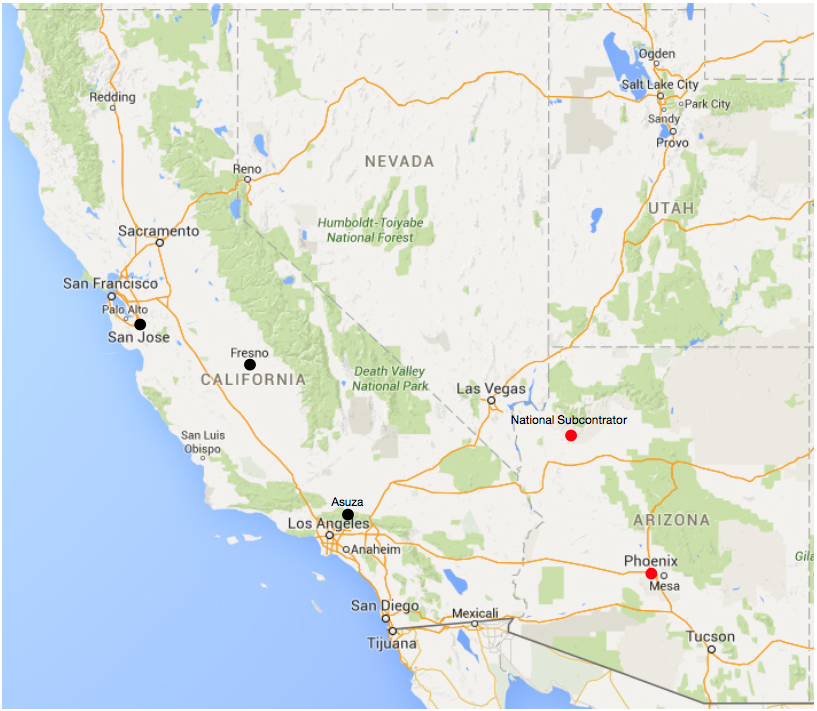
\includegraphics[width=1\textwidth]{img/an-example-delta}
\caption{Map for the problem which indicates warehouses (black dots) and production facilities (red dots).}
\end{figure}

\end{column}
\end{columns}
\end{frame}

%%%%%%%%%%%%%%%%%%%%%%%%%%%%%%%%%%%%%%%%%%%%%%%%%%%%%%%%%%%

\begin{frame}[t]
\frametitle{MANAGEMENT SCIENCE PROCESS}
\framesubtitle{An Example: Delta Hardware Stores}

\begin{columns}[t]
\begin{column}{0.45\textwidth}
\emph{Question}
\vskip0.5cm%
The problem is to determine a \textbf{least cost distribution scheme} of paint produced at its manufacturing plant and shipments from the subcontractor to meet the demands of its California warehouses.
\vskip0.5cm%
\emph{The decision maker is simply being asked;}
\begin{enumerate}
  \item How much paint should be shipped this month from the plant in Phoenix to San Jose, Fresno, and Asuza?
  \item How much extra should be purchased from the subcontractor and sent to each of the three cities to satisfy their orders?
\end{enumerate}
\end{column}

\begin{column}{0.45\textwidth}
\emph{Building the model}
\vskip0.5cm%
\begin{enumerate}
  \item Identify decision variables.
  \item Quantify the objective function.
  \item Write constraints.
  \item Construct a model shell.
  \item Gather data.
\end{enumerate}

\end{column}
\end{columns}
\end{frame}

%%%%%%%%%%%%%%%%%%%%%%%%%%%%%%%%%%%%%%%%%%%%%%%%%%%%%%%%%%%

\begin{frame}[t]
\frametitle{MANAGEMENT SCIENCE PROCESS}
\framesubtitle{An Example: Delta Hardware Stores}

\begin{columns}[t]
\begin{column}{0.45\textwidth}
\emph{Decision Variables}
\vskip0.5cm%
Amount of paint \textbf{shipped} this month;
\begin{description}
  \item [$x_1$] From Phoenix to San Jose
  \item [$x_2$] From Phoenix to Fresno
  \item [$x_3$] From Phoenix to Azusa
\end{description}
\vskip0.5cm%
Amount of paint \textbf{subcontracted} this month;
\begin{description}
  \item [$x_4$] For San Jose
  \item [$x_5$] For Fresno
  \item [$x_6$] For Azusa
\end{description}
\end{column}

\begin{column}{0.45\textwidth}
\emph{Objective Function and Constraints}
\vskip0.5cm%
The objective is to \textbf{minimize the total overall monthly costs} of manufacturing, transporting and subcontracting paint, \textbf{subject to}:
\begin{enumerate}
  \item The Phoenix plant cannot operate beyond its capacity.
  \item The amount ordered from subcontractor cannot exceed a maximum limit.
  \item The orders for paint at each warehouse will be fulfilled.
\end{enumerate}
\end{column}
\end{columns}
\end{frame}

%%%%%%%%%%%%%%%%%%%%%%%%%%%%%%%%%%%%%%%%%%%%%%%%%%%%%%%%%%%

\begin{frame}[t]
\frametitle{MANAGEMENT SCIENCE PROCESS}
\framesubtitle{An Example: Delta Hardware Stores}

\begin{columns}[t]
\begin{column}{0.45\textwidth}
\emph{Parameters}
\vskip0.5cm%
To determine the overall costs;
\begin{description}
  \item [$m$] The manufacturing cost per 10,000 liters of paint at the plant in Phoenix.
  \item [$c$] The procurement cost per 10,000 liters of paint from National Subcontractor
  \item [$t_1, t_2, t_3$] The respective truckload shipping costs form Phoenix to San Jose, Fresno, and Azusa.
  \item [$s_1, s_2, s_3$] The fixed purchase cost per 10,000 liters from the subcontractor to San Jose, Fresno, and Azusa.
\end{description}
\end{column}

\begin{column}{0.45\textwidth}
\vskip0.5cm%
To write to constraints, we need to know;
\begin{description}
  \item [$q_1$] The capacity of the Phoenix plant.
  \item [$q_2$] The maximum number of gallons available from the subcontractor.
  \item [$r_1, r_2, r_3$] The respective orders for paint at the warehouses in San Jose, Fresno, and Azusa.
\end{description}
\end{column}
\end{columns}
\end{frame}

%%%%%%%%%%%%%%%%%%%%%%%%%%%%%%%%%%%%%%%%%%%%%%%%%%%%%%%%%%%

\begin{frame}[t]
\frametitle{MANAGEMENT SCIENCE PROCESS}
\framesubtitle{An Example: Delta Hardware Stores}

\begin{columns}[t]
\begin{column}{0.45\textwidth}
\emph{Objective Function}
\vskip0.5cm%
\begin{equation*}
%\begin{array}{ll@{}ll}
\begin{array}{lll}
\text{Minimize Z}  = & \text{Total Cost} \\
\text{\emph{or}} & & \\
\text{Minimize Z}  = & \text{Manufacturing Cost} \\
                     & + \text{Transportation Cost} \\
                     & + \text{Purchasing Cost} \\
                     & + \text{Subcontracting Cost}\\
\text{\emph{or}} & & \\
\text{Minimize Z}  = & m x_1 + m x_2 + m x_3          \\
                     & + t_1 x_1 + t_2 x_2 + t_3 x_3  \\
                     & + c x_4 + c x_5 + c x_6        \\
                     & + s_1 x_4 + s_2 x_5 + s_3 x_6  \\
\text{\emph{or}} & & \\
\text{Minimize Z}  = & (m + t_1) x_1 + (m+t_2) x_2 + (m+t_3) x_3 \\
                     & + (c + s_1) x_4 + (c + s_2) x_5 + (c + s_3) x_6 \\

%\text{Subject to:} & & \\
%                   & 7D + 3C + 1.5M \leq 2,000 & \text{~warehouse limit for steel} \\
%                   & D \geq 100 & \text{~from contract} \\
%                   & C \leq 500 & \text{~from contract} \\
%                   & D, C, M \geq 0 & \text{~non negativity} \\
%                   & D, C & \text{~are integers}
\end{array}
\end{equation*}
\end{column}

\begin{column}{0.45\textwidth}
\emph{Constraints}
\vskip0.5cm%
The number of truckloads shipped out from Phoenix cannot exceed the plant capacity:
\begin{center}
  $x_1 + x_2 + x_3 \leq q_1$
\end{center}

The number of thousands of gallons ordered from the subcontrator cannot exceed the order limit: 
\begin{center}
  $x_4 + x_5 + x_6 \leq q_2$
\end{center}

The number of thousands of gallons received at each ware- house equals the total orders of the warehouse:
\begin{center}
  $x_1 + x_4  = r_1$ \\
  $x_2 + x_5  = r_2$ \\
  $x_3 + x_6  = r_3$
\end{center}

All shipments must be nonnegative and integer:
\begin{center}
  $x_1, x_2, x_3, x_4, x_5, x_6 \geq 0$ \\
  $x_1, x_2, x_3, x_4, x_5, x_6 : \text{integer}$ 
\end{center}
\end{column}
\end{columns}
\end{frame}

%%%%%%%%%%%%%%%%%%%%%%%%%%%%%%%%%%%%%%%%%%%%%%%%%%%%%%%%%%%

\begin{frame}[t]
\frametitle{MANAGEMENT SCIENCE PROCESS}
\framesubtitle{An Example: Delta Hardware Stores}

\begin{columns}[t]
\begin{column}{0.45\textwidth}
\emph{Model Shell}

\begin{equation*}
\begin{array}{lll}
  \text{Minimize Z}  = & (m + t_1) x_1 + (m+t_2) x_2 + (m+t_3) x_3 \\
                       & + (c + s_1) x_4 + (c + s_2) x_5 + (c + s_3) x_6 \\
  \text{Subject to:}\\
                       & x_1 + x_2 + x_3 \leq q_1 \\
                       & x_4 + x_5 + x_6 \leq q_2 \\
                       & x_1 + x_4  = r_1 \\
                       & x_2 + x_5  = r_2 \\
                       & x_3 + x_6  = r_3 \\
                       & x_1, x_2, x_3, x_4, x_5, x_6 \geq 0 \\
                       & x_1, x_2, x_3, x_4, x_5, x_6 : \text{integer}
\end{array}
\end{equation*}
\end{column}

\begin{column}{0.45\textwidth}
\emph{Data Gathering}
\vskip0.5cm%
Respective orders \\
$r_1$ = 4,000 liters, $r_2$ = 2,000 liters, $r_3$ = 5,000 liters
\vskip0.5cm%
Capacity \\
$q_1$ = 8,000 liters, $q_2$ = 5,000 liters
\vskip0.5cm%
Subcontractor price \\
$c$ = \$5,000 per 1,000 liters
\vskip0.5cm%
Cost of production \\
$m$ = \$3,000 per 1,000 liters 
\vskip0.5cm%
Transportation costs \\
Subcontractor \\
$s_1$ = \$1,200, $s_2$ = \$1,400, $s_3$ = \$1,100 \\
Phoenix Plant \\
$t_1$ = \$1,050, $t_2$ = \$750, $t_3$ = \$650
\end{column}
\end{columns}
\end{frame}

%%%%%%%%%%%%%%%%%%%%%%%%%%%%%%%%%%%%%%%%%%%%%%%%%%%%%%%%%%%

\begin{frame}[t]
\frametitle{MANAGEMENT SCIENCE PROCESS}
\framesubtitle{An Example: Delta Hardware Stores}

\begin{columns}[t]
\begin{column}{0.45\textwidth}
\emph{Mathematical Model}

\begin{equation*}
\begin{array}{lll}
  \text{Minimize Z}  = & 4,050 x_1 + 3,750 x_2 + 3,650 x_3 \\
                       & + 6,200 x_4 + 6,400 x_5 + 6,100 x_6 \\
  \text{Subject to:}\\
                       & x_1 + x_2 + x_3 \leq 8,000 \\
                       & x_4 + x_5 + x_6 \leq 5,000 \\
                       & x_1 + x_4  = 4,000 \\
                       & x_2 + x_5  = 2,000 \\
                       & x_3 + x_6  = 5,000 \\
                       & x_1, x_2, x_3, x_4, x_5, x_6 \geq 0 \\
                       & x_1, x_2, x_3, x_4, x_5, x_6 : \text{integer}
\end{array}
\end{equation*}
\end{column}

\begin{column}{0.45\textwidth}
\emph{Solution Result}
\vskip0.5cm%
$x_1 = 1,000$  liters\\
$x_2 = 2,000$  liters\\
$x_3 = 5,000$  liters\\
$x_4 = 3,000$  liters\\
$x_5 = 0$\\
$x_6 = 0$
\vskip0.5cm%
\emph{Total Cost}
\vskip0.5cm%
\textbf{\$44,800}
\end{column}
\end{columns}
\end{frame}

%%%%%%%%%%%%%%%%%%%%%%%%%%%%%%%%%%%%%%%%%%%%%%%%%%%%%%%%%%%

\begin{frame}[t]
\frametitle{BREAK-EVEN ANALYSIS}
\framesubtitle{Remembrance of an Old Story}

\begin{columns}[t]
\begin{column}{0.45\textwidth}
\textbf{Profit} = Income - Outcome
\end{column}

\begin{column}{0.45\textwidth}
\textbf{Income} = Selling Price per Unit x Number of Units
\vskip0.5cm%
\textbf{Outcome} = Fixed Cost + (Variable Cost per Unit x Number of Units)

\end{column}
\end{columns}
\vskip0.5cm%
\begin{center}

\begin{tikzpicture} [scale=0.9]
  \begin{axis}[%
%    title=Break-Even Analysis - Sample Graph,
    width = 20cm, 
    height = 20cm,
    axis lines=left,
    axis equal image,
    axis on top = true, 
    axis x line = middle, 
    axis y line = middle,
    legend cell align=left,
    legend style={draw=none},
    xmin = 0, xmax = 31, 
    ymin = 0, ymax = 21,
    xticklabels={,,},
    yticklabels={,,},
%    /pgfplots/xtick = {0,10,...,40},
%    /pgfplots/ytick = {0,10,...,40},
%    tick align = outside,
    xlabel = {\emph{Production Volume (unit)}},
    x label style={
      at={(axis description cs:0.88,-0.05)},
      anchor=north,
    },
    ylabel = {\emph{Revenue and Cost (\$)}},
    ylabel style = {
      at={(axis description cs:-0.05,0.84)},
      rotate=90,   
      anchor=south,
    },
    xtick={12},
    xticklabels={$n$},
    ytick={7.9},
    yticklabels={$a$},
    ]%
    % INCOME LINE
    \addplot[%
    green!100,
    line width = 1.5,
    name path=Income
    ]%
    coordinates {(0,0)(26,17)}
    node [above right,rotate=0,black] {Income};
    % TOTAL COST LINE
    \addplot[%
    red!100,
    line width = 1.5,
    name path=TotalCost
    ]%
    coordinates {(0,6)(26,10)}
    node [above,rotate=0,black] {Total Cost (Outcome)};
    % FIXED COST LINE
    \addplot[%
    red!100,
    dashed,
    line width = 1,
    name path=FixedCost
    ]%
    coordinates {(0,6)(26,6)}
    node [above right,rotate=0,black] {Fixed Cost};
    % VARIABLE COST LINE
    \addplot[%
    red!100,
    dashed,
    line width = 1,
    name path=VariableCost
    ]%
    coordinates {(0,0)(26,4)}
    node [above right,rotate=0,black] {Variable Cost};

    % POINTS
    \addplot[%
    black!100,
    dotted,
    line width = 1,
    name path=BreakEvenAxisY
    ]%
    coordinates {(12,8)(12,0)};

    \addplot[%
    black!100,
    dotted,
    line width = 1,
    name path=BreakEvenAxisX
    ]%
    coordinates {(12,7.9)(0,7.9)};

    % INTERSECTION OF TWO LINES
    \path [name intersections={of=Income and TotalCost,by=E}];
    \node [fill=black,circle,label=Break-Even Point] at (E) {};
  \end{axis}

\end{tikzpicture}

\end{center}
\end{frame}

%%%%%%%%%%%%%%%%%%%%%%%%%%%%%%%%%%%%%%%%%%%%%%%%%%%%%%%%%%%

\begin{frame}[t]
\frametitle{TABLE TALK PROBLEMS FROM TEXTBOOK}
\framesubtitle{Introduction to Management Science}

\begin{columns}[t]
\begin{column}{0.45\textwidth}
\emph{Problem -- Break-Even Analysis}
\vskip0.5cm%
Three types of manufacturing equipment for engine gaskets are under consideration. Their fixed costs and resulting variable costs per unit are shown in the table below.
\begin{table}
\begin{tabular}{p{0.33\textwidth}p{0.33\textwidth}p{0.33\textwidth}}
  \hline
              & \emph{Fixed Cost (\$)} & \emph{Variable Cost (\$/unit)} \\
  \hline
  Equipment A & 4,000  & 1.90 \\
  Equipment B & 7,000  & 1.40\\
  Equipment C & 12,000 & 1.00\\
  \hline
\end{tabular}
\end{table}

\begin{enumerate}
  \item At what volume of production would Equipment A and Equipment B cost the same?
  \item Establish this breakeven point for equipments B and C.
  \item Suppose the volume anticipated was 8,000 units. Which equipment should be purchased?
  \item Suppose the volume anticipated was 12,900 units. Which equipment should then be purchased?
\end{enumerate}
\end{column}

\begin{column}{0.45\textwidth}
\emph{Problem -- Break-Even Analysis}
\vskip0.5cm%
Two brothers want to open a small neighborhood bakery, where they will specialize in loaves of bread. They have carefully estimated their fixed costs to be \$110,000 per year. This includes a salary of \$35,000 for each brother.
\vskip0.5cm%
The facility they will use is a former pizza kitchen. One problem is that there is limited capacity, so there will be an upper limit on the number of loaves of bread they can produce.
\vskip0.5cm%
Baking 6 days a week, the brothers believe they can produce 150 loaves per day. The cost to them for each loaf is \$0.55. They believe they will be able to sell all the bread they can bake. They plan to bake 312 days during the year.

\begin{enumerate}
  \item Given these projections, how much will the brothers have to charge per loaf to stay in business?
  \item Suppose they are willing to take a much lower salary to get their business started. If they each agreed to take only \$25,000 per year, how much would they have to charge for their bread?
\end{enumerate}
\end{column}
\end{columns}
\end{frame}

%%%%%%%%%%%%%%%%%%%%%%%%%%%%%%%%%%%%%%%%%%%%%%%%%%%%%%%%%%%

%\begin{frame}[t]
%\frametitle{INDEPENDENCE}
%\framesubtitle{Freedom}
%
%\begin{columns}[t]
%\begin{column}{0.45\textwidth}
%\vskip0.5cm%
%\end{column}
%
%\begin{column}{0.45\textwidth}
%\vskip0.5cm%
%\end{column}
%\end{columns}
%\end{frame}

%%%%%%%%%%%%%%%%%%%%%%%%%%%%%%%%%%%%%%%%%%%%%%%%%%%%%%%%%%%

\end{document}